%! 2theta-omega scans
\begin{figure}
    \centering
    \includegraphics{1_pressure_2theta_labeled.pdf}
    \caption{\thetaomega-patterns of \cro\ thin films deposited on \textit{m}-plane sapphire for various oxygen partial pressures.
    The solid lines indicate (30.0) substrate reflections corresponding to copper radiation, whereas the dashed lines indicate (30.0) substrate reflections corresponding to tungsten radiation.}
    \label{Fig:Results_1_pressure_2theta}
\end{figure}
In the following, the results for the samples produced at four different oxygen partial pressures are analyzed.
In Fig.\,\ref{Fig:Results_1_pressure_2theta}, the \thetaomega-patterns are depicted.
For each pattern, the two peaks (solid line) at around \qty{68}{\degree} correspond to the (30.0) reflection of the \textit{m}-plane oriented sapphire substrate.
The splitting occurs due to the similar wavelength of \ce{Cu}-K\textalpha\textsubscript{1} and \ce{Cu}-K\textalpha\textsubscript{2} radiation.
The additional peaks also stem mainly from the (30.0) reflection of \ce{Al2O3} and are caused by
\ce{W}-L\textbeta\textsubscript{2}-,
\ce{W}-L\textbeta\textsubscript{1}-,
\ce{Cu}-K\textbeta-,
\ce{W}-L\textalpha\textsubscript{1}- and
\ce{W}-L\textalpha\textsubscript{2}-radiation (increasing angles).
In the vicinity of the calculated peak position for the (30.0) reflection of \cro\ (cf.~\ref{tab:d_strained}), there is a peak observed for each sample, indicating that the \textalpha-phase of \cro\ is present.
Note that the peak position is varying depending on the chosen oxygen partial pressure.
The difference to the expected peak position $2\theta_0$ is expressed as \gls{oop}\ strain $\epsilon_{zz}$ using the Bragg equation \eqref{Equ:Theory_BraggCondition} and then
\begin{equation}
    \label{Equ:Results_oop_strain_def}
    \epsilon_{zz}
    =\frac{d-d_0}{d_0}
    =\left(\frac{1}{\sin(2\theta/2)}-\frac{1}{\sin(2\theta_0/2)}\right)
    \cdot\sin(2\theta_0/2)\,.
\end{equation}
In Fig.\,\ref{Fig:Results_1_pressureTemperature_yyaxis_strainOmega}a, the calculated strain is shown in dependence of the corresponding oxygen partial pressure (black circles).
The strain decreases from approx.\ \qty{0.95}{\percent} to \qty{0.45}{\percent} with increasing pressure.
This strain reduction may therefore be the result of increased background gas scattering which results in less kinetic energy of the specimen reaching the heated substrate (cf.~\ref{Sec:Methods_pld}).
% \begin{figure}
%     \centering
%     \begin{tabular}{ll}
%         \textbf{(a)}&\textbf{(b)} \figSpace\\
%         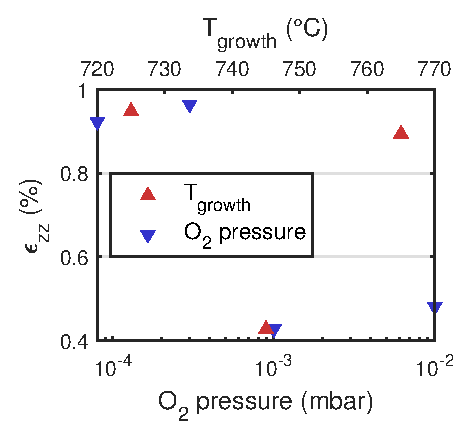
\includegraphics[align=c]{1_both_strain.eps}    
%         &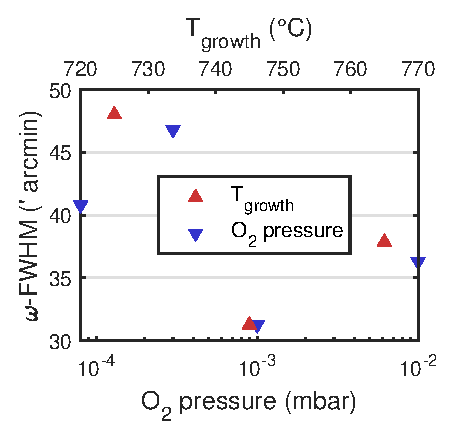
\includegraphics[align=c]{1_both_FWHM.eps}
%     \end{tabular}
%     \caption{
%         \textbf{(a)} \gls{oop}\ strain calculated with \eqref{Equ:Results_oop_strain_def} and \textbf{(b)} \textomega-FWHMs for samples from growth temperature series (red triangles, top \textit{x}-axis) and oxygen partial pressure series (blue triangles, bottom \textit{x}-axis).
%         }
%     \label{Fig:Results_1_both_strainFWHM}
% \end{figure}
\begin{figure}
    \centering
    \begin{tabular}{ll}
        \textbf{(a)} & \textbf{(b)} \figSpace\\
        \includegraphics[align=c]{1_pressure_strainOmega.pdf}  \hfill  
        &\includegraphics[align=c]{1_temperature_strainOmega.pdf}
    \end{tabular}
    \caption{
        \textbf{(a)} Out-of-plane Strain and \textomega-FWHM for the samples fabricated at different oxygen pressures.
        \textbf{(b)}~Out-of-plane Strain and \textomega-FWHM for the samples fabricated at different growth temperatures.
    }
    \label{Fig:Results_1_pressureTemperature_yyaxis_strainOmega}
\end{figure}


%! omega-scans
For each sample, the $2\theta$ angle was fixed to the observed (30.0) reflection of \cro\ and an \textomega-scan was performed.
The \gls{FWHM} of the \textomega-patterns (henceforth \emph{\textomega-FWHM}) are depicted in
    Fig.\,\ref{Fig:Results_1_pressureTemperature_yyaxis_strainOmega}a (orange triangles).
The values vary between approx.\ \qtylist{30;50}{\arcminute} and show a dependence on oxygen partial pressure, which is less pronounced compared with \gls{oop}\ strain.
Still, since \textomega-FWHM is connected to the mosaicity of the thin film, higher oxygen partial pressures yield slightly better crystal qualities.
Note that due to the fact that an oxygen partial pressure of \qty{1e-3}{\milli\bar} yielded the best crystal quality, this value is used for future deposition processes.

%! phi-scan
To probe for rotational domains of the thin films, \textphi-scans were performed by fixing $2\theta$ and $\omega$ to the corresponding angles of the (30.6) plane of \cro, which has an inclination angle of \qty{32.4}{\degree} with respect to the (30.0) plane.
The diffraction patterns are depicted in Fig.\,\ref{Fig:Results_1_phiScan}.
The observed peaks of the thin film align with the peaks of the single crystal substrate, indicating that the film has no in-plane rotation with respect to the substrate.
Furthermore, the absence of additional peaks indicates that there exists only a single domain of the thin film.
\begin{figure}
    \centering
    \includegraphics{1_both_phi_oneSub.pdf}
    \caption{
        Diffraction patterns of \textphi-scans performed on the inclined (30.6) reflection for \textit{m}-plane oriented \cro\ samples (color).
        The corresponding pattern of the \alo\ substrate is also depicted (black).
        The diffraction patterns cover the samples from variation of oxygen partial pressure (teal to blue colored) and variation of growth temperature (red to yellow colored).
    }
    \label{Fig:Results_1_phiScan}
\end{figure}

%! growth rates
The growth rate $g$ varies between \qtylist{3;7}{\pm\per\pulse} and is depicted in Fig.\,\ref{Fig:Results_1_pressureTemperature_growthrate}a.
No systematic dependence on the oxygen partial pressure can be observed.
This is not expected, because the background pressure is related to scattering of the plasma species, which should alter the kinetic energy and therefore the growth dynamics.
This behavior is attributed to reduced laser fluence on the target due to window coating, as it will be explained below.
\begin{figure}
    \centering
    \begin{tabular}{lcl}
        \textbf{(a)} &\hfill& \textbf{(b)} \figSpace\\
        \includegraphics[align=c]{1_pressure_growthrate.pdf} &
        &\includegraphics[align=c]{1_temperature_growthrate.pdf}
    \end{tabular}
    \caption{
        Growth rates $g$ for the samples fabricated with \textbf{(a)} varying oxygen pressure and \textbf{(b)} varying growth temperature.
    }
    \label{Fig:Results_1_pressureTemperature_growthrate}
\end{figure}
% \begin{figure}
%     \centering
%     \begin{tabular}{ll}
%         \textbf{(a)} & \textbf{(b)} \figSpace\\
%         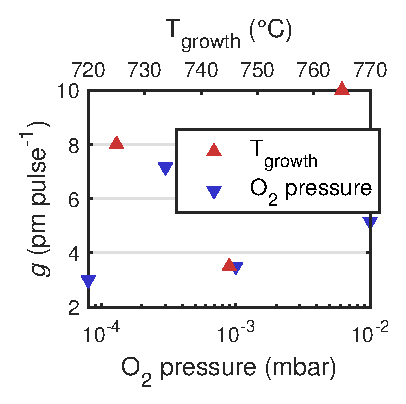
\includegraphics[align=c]{1_both_growthrate.eps}
%         &\includegraphics[align=c]{camera_initial.eps}
%     \end{tabular}
%     \caption{
%         \textbf{(a)} Growth rates $g$ for samples from growth temperature series (red triangles, top \textit{x}-axis) and oxygen partial pressure series (blue triangles, bottom \textit{x}-axis).
%         \textbf{(b)} Image of the samples produced at different oxygen partial pressures ($T=\qty{740}{\degreeCelsius}$) and different growth temperatures ($p(\mathrm{O_2})=\qty{1e-3}{\milli\bar}$).
%         }
%     \label{Fig:Results_1_growthRates_photograph}
% \end{figure}

%! Transmission
The transmission spectra of two selected \cro\ thin films are shown in Fig.\,\ref{Fig:Results_1_transmission}a.
The samples are not fully transparent in the visible spectrum (\qty{80}{\percent} transmission at \qty{400}{\nm}) and they exhibit a green tint, as can also be seen in Fig.\,\ref{Fig:Results_1_samplesPhoto}.
% fitting with indirect gap: cheng 1996, al-kuhaili2007 (^1/2)
% fitting with direct gap: farrell 2015 (^2)
% mi2018 states cr2o3 is a direct bandgap semiconductor
To determine the onset of absorption $E_\mathrm{opt}$, an $\alpha^2$ vs.\ $E$ plot (Fig.\,\ref{Fig:Results_1_transmission}b) is utilized (cf.~\ref{Sec:Methods_transmission}).
Although the publications used for reference in this work support the direct transition nature of \cro\ 
    \cite{farrell2015,mi2018},
it has to be noted that there exist studies determining the optical band gap of \cro\ by assuming an indirect transition nature 
    \cite{cheng1996,al-kuhaili2007}.
However, all of them utilize a \textsc{Tauc} plot $(\alpha E)^\eta$ vs.\ $E$, which is an unappropriate method for crystalline solids as discussed in~\ref{Sec:Methods_transmission}.
Therefore, the method based on the assumption of parabolic shape of bands as well as direct transitions (cf.\ \ref{Sec:Methods_transmission}) is used.
Fitting the linear regime between \qtylist{3.75;4.3}{\eV} results in $E_\mathrm{opt}\approx\qty{3.6}{\eV}$ for both samples, which differ in strain and \textomega-FWHM by a factor of approx.\ 2 and 0.3, respectively.
A second absorption edge can be identified between \qtylist{5.3;5.5}{\eV} and yields an optical gap of $E_\mathrm{opt}\approx\qty{5.1}{\eV}$ for both samples.
\begin{figure}
    \centering
    \begin{tabular}{c}
        \multicolumn{1}{l}{\textbf{(a)}}\figSpace\\
        \includegraphics[align=t]{1_pressure_transmission.pdf}\figSpace\\
        \multicolumn{1}{l}{\textbf{(b)}}\figSpace\\
        \includegraphics[align=t]{1_pressure_tauc.pdf}
    \end{tabular}
    \caption{\textbf{(a)} Transmission spectra of two selected \cro\ thin films, deposited with different oxygen partial pressures of \qtylist{1e-3;8e-5}{\milli\bar}.
    The spectra are normalized to a corresponding uncoated \textit{m}-plane sapphire substrate.
    No correction to film thickness was done, which results in a lower transmittance of the thicker sample (purple).
    \textbf{(b)}~$\alpha^2$ vs.\ $E$ plot of the above-mentioned samples.
    It is assumed that \cro\ has a direct bandgap
        \cite{farrell2015,mi2018}.
    The fitting regime for determining the optical gap is chosen to be between \qtylist{3.75;4.3}{\eV}, as well as between \qtylist{5.3;5.5}{\eV}.
    }
    \label{Fig:Results_1_transmission}
\end{figure}